\subsection{A controlled quadrupole-coupling path}

To isolate a dynamical origin, we varied the $^{135}$Ba quadrupole coupling as
$\Gamma_0=0.6s$ MeV, with $s=0,0.25,0.50,0.75,1$, while keeping the exchange
and monopole strengths, core, occupation and charge operator fixed.
These are interventions in the model, not alternative fits to the nucleus.
Forward and backward maximum-overlap tracking both select the lowest
$11/2$ state throughout the sampled path. Adjacent squared overlaps exceed
0.907, and the smallest sampled gap to the next state of the same spin is
0.481 MeV. Thus no lowest-state switch is observed at this resolution.

Figure~\ref{fig:path} shows a strong redistribution with little change in total
strength. Complete $q_2$ remains between 0.67662 and
$0.69413\,e^2{\rm b}^2$, a range of less than $2.6\%$, and
$\langle n_d\rangle$ stays between 2.324 and 2.354. The static fraction,
however, rises from $0.0091\%$ to $33.69\%$. The core-$R=2$ probability
increases from 0.0151 to 0.4837, while the core-$R=0$ probability falls
from 0.9522 to 0.4886. In this controlled comparison, quadrupole coupling
principally changes angular recoupling and static polarization rather than
the amount of quadratic charge strength.

\begin{figure*}[t]
\centering
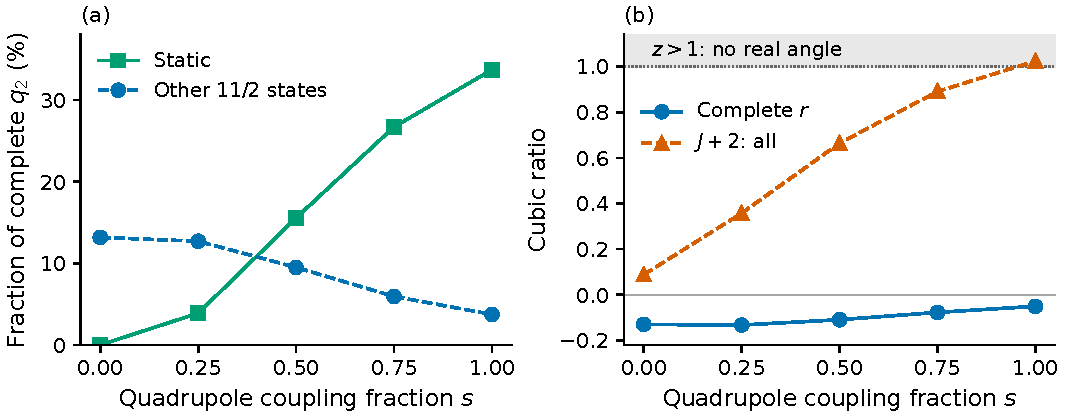
\includegraphics[width=\textwidth]{figures/quadrupole_path-v2.pdf}
\caption{Fixed-exchange/monopole control for $^{135}$Ba:
$\Gamma_0=0.6s$ MeV, $\Lambda_0=1$ MeV, $A_0=-0.9$ MeV.
The core and electric-quadrupole operator are unchanged.
(a) Static and other-same-spin fractions of complete $q_2$.
(b) Complete signed ratio and the all-$15/2$ selected ratio.
Points are the five calculated settings; lines guide the eye.
The shaded region has no real selected angle.}\label{fig:path}
\end{figure*}

The selected ratio rises through a specific change of its numerator and
denominator. Over the path, $S_\infty$ falls from 2.32070 to
$1.62594\,e^2{\rm b}^2$, whereas the signed chain $C_\infty$ grows from
0.37162 to $2.53787\,e^3{\rm b}^3$. In the intermediate energy eigenbasis,
its middle-diagonal contribution changes from
$-0.73467$ to $+1.16709\,e^3{\rm b}^3$: cancellation with off-diagonal
paths is replaced by reinforcement. Consequently $z_\infty$ rises from
0.08795 to 1.02414. At the final point, the additional spin sectors in the
complete cubic moment still largely cancel. Since the all-$15/2$ projector
is unchanged along this path, the result is a change of the initial
state's charge response, not a consequence of reordering a five-state list.

\subsection{Operator sensitivity}

We evaluated seven operator/calibration settings on each fixed state: the primary operator; $e_F=0.0625$ and $0.25\,e\,{\rm b}$; $\chi'=0$ and $\chi'=\chi$; and the lower and upper quoted-margin core-strength endpoints. Each alternate $\chi'$ was recalibrated to the same core $B(E2)$, with no fit to the complete--restricted difference. These 35 calculations are deterministic sensitivity tests, not samples from an operator posterior. In particular, the $^{128}$Ba strength margin propagated from the quoted half-life is not a complete uncertainty, and cross-isotope covariance is unavailable.

Across these settings, $q_2$ decreases at every isotope step, the complete $15/2$ channel contains only $14.12$--$29.24\%$ of full quadratic strength, and its first five states contain $99.588$--$99.939\%$ of that channel. The distinction between channel saturation and full coverage therefore persists. The particular cubic coordinates are more operator dependent.

For $^{135}$Ba, $z_\infty>1$ survives both tested fermion charges and both calibration endpoints. It does not survive the alternate $\chi'$ operators. With $\chi'=0$, the complete and selected-all folded angles are $24.418^\circ$ and $6.241^\circ$; with $\chi'=\chi=-0.24$, they are $20.166^\circ$ and $10.659^\circ$. Full cubic signs and some isotope-angle trends also change. Thus the out-of-domain event is a property of the primary operator and the tested nearby charge settings, while the broader separation of complete and selected-channel information remains. None of these operator substitutions changes the underlying eigenstate.

\subsection{Static-moment constraints and calibration alternatives}

The numerical closure checks do not establish the accuracy of the predicted
electromagnetic network. An additional check uses signed spectroscopic moments,
$Q_s(J)=\sqrt{16\pi/5}\langle J,J|T_{20}|J,J\rangle$.
For $^{137}$Ba, the calculation gives
$Q_s(11/2^-)=+0.77296\,e\,{\rm b}$, consistent with the evaluated
$+0.78(9)\,e\,{\rm b}$ \cite{ENSDF}. This is a consistency check at the
source-named charge-calibration target, rather than an independent test.

The comparison is less favorable for the state with the largest channel
redistribution. For $^{135}$Ba, our prediction is
$+1.17693\,e\,{\rm b}$, whereas Ref.~\cite{Nomura2017} quotes
$+0.98(8)\,e\,{\rm b}$ experimentally and $+1.13\,e\,{\rm b}$ in its
calculation. The archived adopted value is $+0.96(8)\,e\,{\rm b}$;
these evaluated and paper-quoted values are retained separately.
Our result therefore overpredicts the static polarization.
For the $^{136}$Ba $2_1^+$ calibration state, the calculated
$-0.30324\,e\,{\rm b}$ must also be compared with branch-dependent
evaluated alternatives, including $-0.19(6)$ and $+0.07(7)\,e\,{\rm b}$,
whose original numerical role in the source calibration is unspecified.
For this primary comparison, we do not select a branch or refit the operator
to improve the agreement.
The mechanism established by the coupling path is consequently a property
of this model family; the quantitative redistribution in the actual
$^{135}$Ba state requires further electromagnetic constraints.

We therefore also reconstructed the two source-named moment calibrations
without changing either Hamiltonian. For each distinct central
$^{136}$Ba $2_1^+$ moment target, we solved for $\chi'$ with positive $e_B$
recalibrated to the same core $B_\uparrow=0.407\,e^2{\rm b}^2$,
then determined $e_F$ from $Q_s(^{137}{\rm Ba})=0.78\,e\,{\rm b}$.
All finite sign-consistent roots were retained. The $^{135}$Ba moment
was not used in these equations; its boson charge was recalibrated to
the unchanged $^{134}$Ba strength.

\begin{table}[t]
\caption{Conditional moment calibrations with fixed Hamiltonians.
$t_{136}$ is the core moment target; $e_F$ and $Q_s(135)$ are in
$e\,{\rm b}$. Ratios refer to the lowest $^{135}$Ba $11/2^-$ state.
Both $|r|>1$ and $z_\infty>1$ imply an undefined real angle.}\label{tab:calibrated}
\centering
\setlength{\tabcolsep}{3pt}
\begin{tabular}{rrrrrr}
\toprule
$t_{136}$ & $\chi'$ & $e_F$ & $Q_s(135)$ & $r$ & $z_\infty$\\
\midrule
$-0.19$ & 0.982 & 0.199 & 1.089 & $-0.642$ & 1.030\\
$+0.01$ & 1.959 & 0.311 & 0.923 & $-1.093$ & 0.850\\
$+0.02$ & 2.004 & 0.317 & 0.915 & $-1.096$ & 0.840\\
$+0.07$ & 2.222 & 0.344 & 0.873 & $-1.092$ & 0.792\\
$+0.25$ & 2.943 & 0.445 & 0.723 & $-0.920$ & 0.640\\
\bottomrule
\end{tabular}
\end{table}

The $+0.01$ and $+0.02\,e\,{\rm b}$ targets give $^{135}$Ba predictions
within the quoted $0.08\,e\,{\rm b}$ margin of 0.96.
However, their complete signed ratios are below $-1$, so even the complete
moment cannot be converted to a real rigid-equivalent angle
(Table~\ref{tab:calibrated}). The independent E2 parameter $\chi'$ is not
restricted here by a customary range for the Hamiltonian's $\chi$.
These are conditional central-value calibrations: moment and strength
branches can covary, the averaged core strength was held fixed, and the
135/137Ba moment evaluations share source lineage.
No branch was selected by its $^{135}$Ba agreement and no posterior
preference is inferred.

Spectral truncation can also affect a marginal domain crossing.
For $^{137}$Ba with the $+0.01\,e\,{\rm b}$ core target,
$z_5=1.00027$ but $z_\infty=0.99484$; completing the selected spin
restores its real angle, while the complete ratio remains
$r=-1.08957$. Thus the spectral cutoff, angular-channel coverage and
moment-to-shape conversion require separate checks.
An additional static-moment match through $\Gamma_0$ alone retains
a large complete--selected separation but shifts the calculated spectrum;
Appendix~\ref{app:momentmatch} gives that conditional control.
